\documentclass{prova}

\usepackage{amssymb}
\usepackage{gensymb}

\renewcommand{\sin}{\mbox{sen}}
\newcommand{\ra}{\rightarrow}
\newcommand{\lra}{\leftrightarrow}
\newcommand{\Ra}{\Rightarrow}
\newcommand{\LRa}{\Leftrightarrow}
\renewcommand{\lnot}{\sim}
\newcommand{\larg}{\vdash}
\newcommand{\ds}{\displaystyle}
\newcommand{\sen}{\mathop\mathrm{sen}\nolimits}
\newcommand{\tg}{\mathop\mathrm{tg}\nolimits}

\professor{Prof. Adriano Barbosa}
\disciplina{Introdução ao Cálculo}
\avaliacao{P4}
\curso{Matem\'atica}
\data{02/10/2020}

\begin{document}
    \cabecalho{5}  % o numero 5 indica a qnt de quadros na tabela de nota
    
    \textbf{Todas as respostas devem ser justificadas.}
    \begin{questionario}
	\q{Sabendo que $\sen x + \cos x = 0,9$, determine o valor de $\sen x
	   \cdot \cos x$.}
	%\q{Sabendo que $\ds\sec x + \tg x= 1,5$, determine os valores
	%   de $\sen x$ e $\cos x$.}
	\q{Certa vez, um professor pediu para que sua turma calculasse a soma
	   dos números de 1 a 100 e Gauss (1777 -- 1855), que ainda era uma
	   criança, resolveu o problema surpreendentemente rápido e de forma
	   muito simples e criativa. Ele observou que somando a primeira
	   parcela com a última ou a segunda com a penúltima o resultado era
	   igual a 101, pois enquanto uma parcela cresce uma unidade a outra
	   diminui uma unidade. Dessa forma, o resultado final da soma pedida
	   pelo professor era igual a $50\times 101 = 5050$.}
	\begin{figure}[h]
	    \centering
	    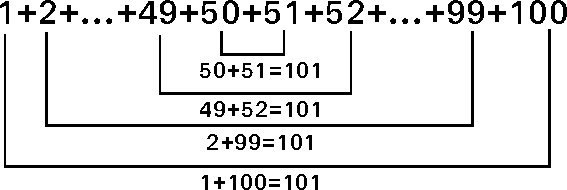
\includegraphics[width=0.3\textwidth]{fig2.pdf}
	\end{figure}

	Determine o valor da soma $\cos^2 1\degree + \cos^2 2\degree +
	\cdots + \cos^2 89\degree$.
	%Lembre que $\ds\sen\left(90\degree-x\right) = \cos x$.
	\q{Determine a medida do segmento $\overline{AD}$.}
	\begin{figure}[h]
	    \centering
	    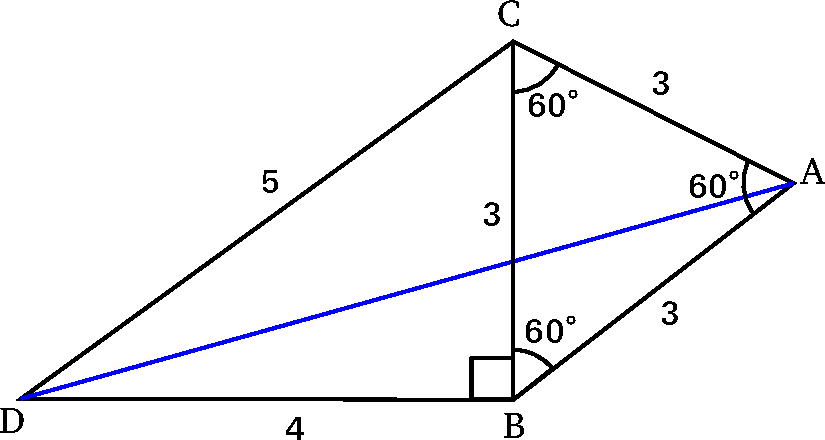
\includegraphics[width=0.5\textwidth]{fig1.pdf}
	\end{figure}
	\q{Calcule o limite $\ds\lim_{x\rightarrow -4}
	   \frac{\sqrt{x^2+9}-5}{x+4}$ sem usar tabelas.} 
	\q{Calcule o limite $\ds\lim_{x\rightarrow -3}
	   \frac{x^2-9}{2x^2+7x+3}$ sem usar tabelas.}
    \end{questionario}
\end{document}
